\section{Auswertung}
\label{sec:Auswertung}

% Messwerte: Alle gemessenen physikalischen Größen sind übersichtlich darzustellen.

% Auswertung:
% Berechnung der geforderten Endergebnisse
% mit allen Zwischenrechnungen und Fehlerformeln, sodass die Rechnung nachvollziehbar ist.
% Eine kurze Erläuterung der Rechnungen (z.B. verwendete Programme)
% Graphische Darstellung der Ergebnisse

\begin{figure}
    \centering
    \begin{subfigure}{0.3\textwidth}
        \centering
        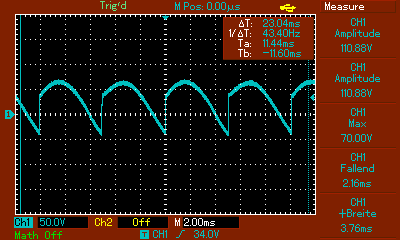
\includegraphics[width=\textwidth]{images/1_0.png}
        \caption{$\varphi = \SI{0}{\degree}$}
        \label{fig:1_0}
    \end{subfigure}
    \begin{subfigure}{0.3\textwidth}
        \centering
        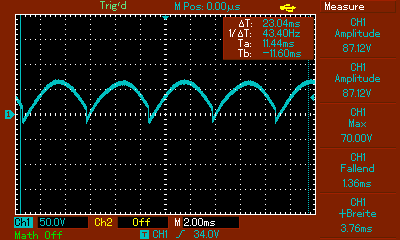
\includegraphics[width=\textwidth]{images/1_45.png}
        \caption{$\varphi = \SI{45}{\degree}$}
        \label{fig:1_45}
    \end{subfigure}
    \begin{subfigure}{0.3\textwidth}
        \centering
        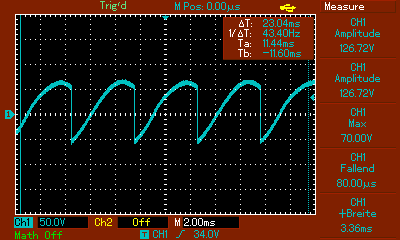
\includegraphics[width=\textwidth]{images/1_90.png}
        \caption{$\varphi = \SI{90}{\degree}$}
        \label{fig:1_90}
    \end{subfigure}
    \par\medskip % Vertikaler Platz
    \begin{subfigure}{0.3\textwidth}
        \centering
        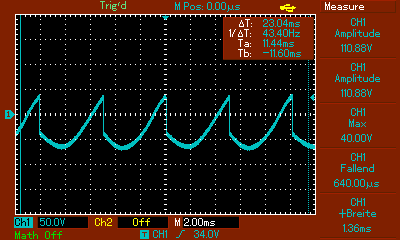
\includegraphics[width=\textwidth]{images/1_180.png}
        \caption{$\varphi = \SI{180}{\degree}$}
        \label{fig:1_180}
    \end{subfigure}
    \begin{subfigure}{0.3\textwidth}
        \centering
        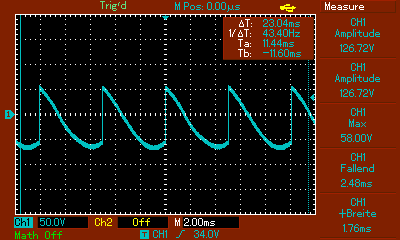
\includegraphics[width=\textwidth]{images/1_270.png}
        \caption{$\varphi = \SI{270}{\degree}$}
        \label{fig:1_270}
    \end{subfigure}
    \caption{Screenshots der Spannung ohne zwischengeschaltetem Noise-Generator bei verschiedenen Phasenverschiebungen $\varphi$}
    \label{fig:1}
\end{figure}

\begin{figure}
    \centering
    \begin{subfigure}{0.3\textwidth}
        \centering
        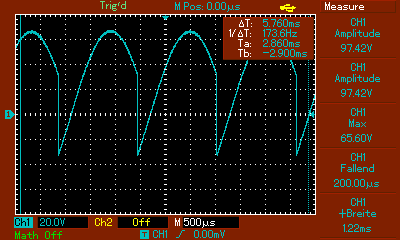
\includegraphics[width=\textwidth]{images/2_0.png}
        \caption{$\varphi = \SI{0}{\degree}$}
        \label{fig:2_0}
    \end{subfigure}
    \begin{subfigure}{0.3\textwidth}
        \centering
        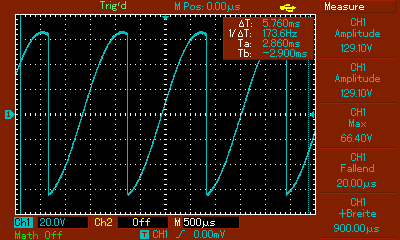
\includegraphics[width=\textwidth]{images/2_45.png}
        \caption{$\varphi = \SI{45}{\degree}$}
        \label{fig:2_45}
    \end{subfigure}
    \begin{subfigure}{0.3\textwidth}
        \centering
        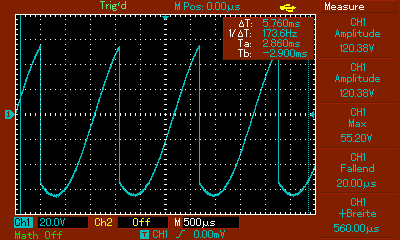
\includegraphics[width=\textwidth]{images/2_90.png}
        \caption{$\varphi = \SI{90}{\degree}$}
        \label{fig:2_90}
    \end{subfigure}
    \par\medskip % Vertikaler Platz
    \begin{subfigure}{0.3\textwidth}
        \centering
        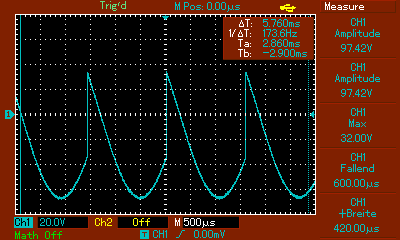
\includegraphics[width=\textwidth]{images/2_180.png}
        \caption{$\varphi = \SI{180}{\degree}$}
        \label{fig:2_180}
    \end{subfigure}
    \begin{subfigure}{0.3\textwidth}
        \centering
        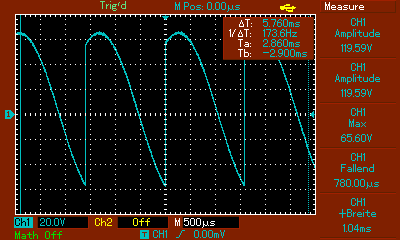
\includegraphics[width=\textwidth]{images/2_270.png}
        \caption{$\varphi = \SI{270}{\degree}$}
        \label{fig:2_270}
    \end{subfigure}
    \caption{Screenshots der Spannung mit zwischengeschaltetem Noise-Generator bei verschiedenen Phasenverschiebungen $\varphi$}
    \label{fig:2}
\end{figure}